\section{Overview}
\subsection{Purpose}
This document contains pertinent information for the architecture and
implementation of Acme Corporation's network upgrade, including details over 
topology, services, and high-level configuration descriptions where applicable.
\subsection{Services}
All existing services must be upgraded to accommodate the network upgrade. 
The scope of each service upgrade will vary based on the need, but each
service will be reimplemented to better fit within the post-upgrade network 
architecture. 
\subsubsection{Existing Services}
The following existing services will be upgraded (in no particular order):
\newcolumntype{P}[1]{>{\centering\arraybackslash}p{#1}}
\begin{center}
\begin{tabular}{|P{7.3cm}|P{5.5cm}|}
    \hline
    \textbf{Service Description} & \textbf{Preferred Package/Application} \\
    \hline
    Network File System (NFS) & nfs-kernel-server, nfs-client \\
    \hline
    Webserver & apache2 \\
    \hline
    Database & mariadb \\
    \hline
    Email & ??? \\
    \hline
    Active Directory (AD) & openldap \\
    \hline
    Domain Name Server (DNS) & \textcolor{red}{-\$30,000} \\
    \hline
    Dynamic Host Configuration Protocol (DHCP) & dhcpd \\
    \hline
\end{tabular}
\end{center}
\subsubsection{New Services}
The following new services will be implemented on the network (in no particular
order):
\newcolumntype{P}[1]{>{\centering\arraybackslash}p{#1}}
\begin{center}
\begin{tabular}{|P{7.3cm}|P{5.5cm}|}
    \hline
    \textbf{Service Description} & \textbf{Preferred Package/Application} \\
    \hline
    Virtual Local Area Network (VLAN) & vlan \\
    \hline
    Configuration Management & puppet \\
    \hline
    Monitoring & nagios \\
    \hline
    Virtual Private Network (VPN) & openvpn \\
    \hline
\end{tabular}
\end{center}
\subsection{Architecture}
\subsubsection{Architecture Overview}
\subsubsection{Network Topology}
\begin{figure}[h!]
	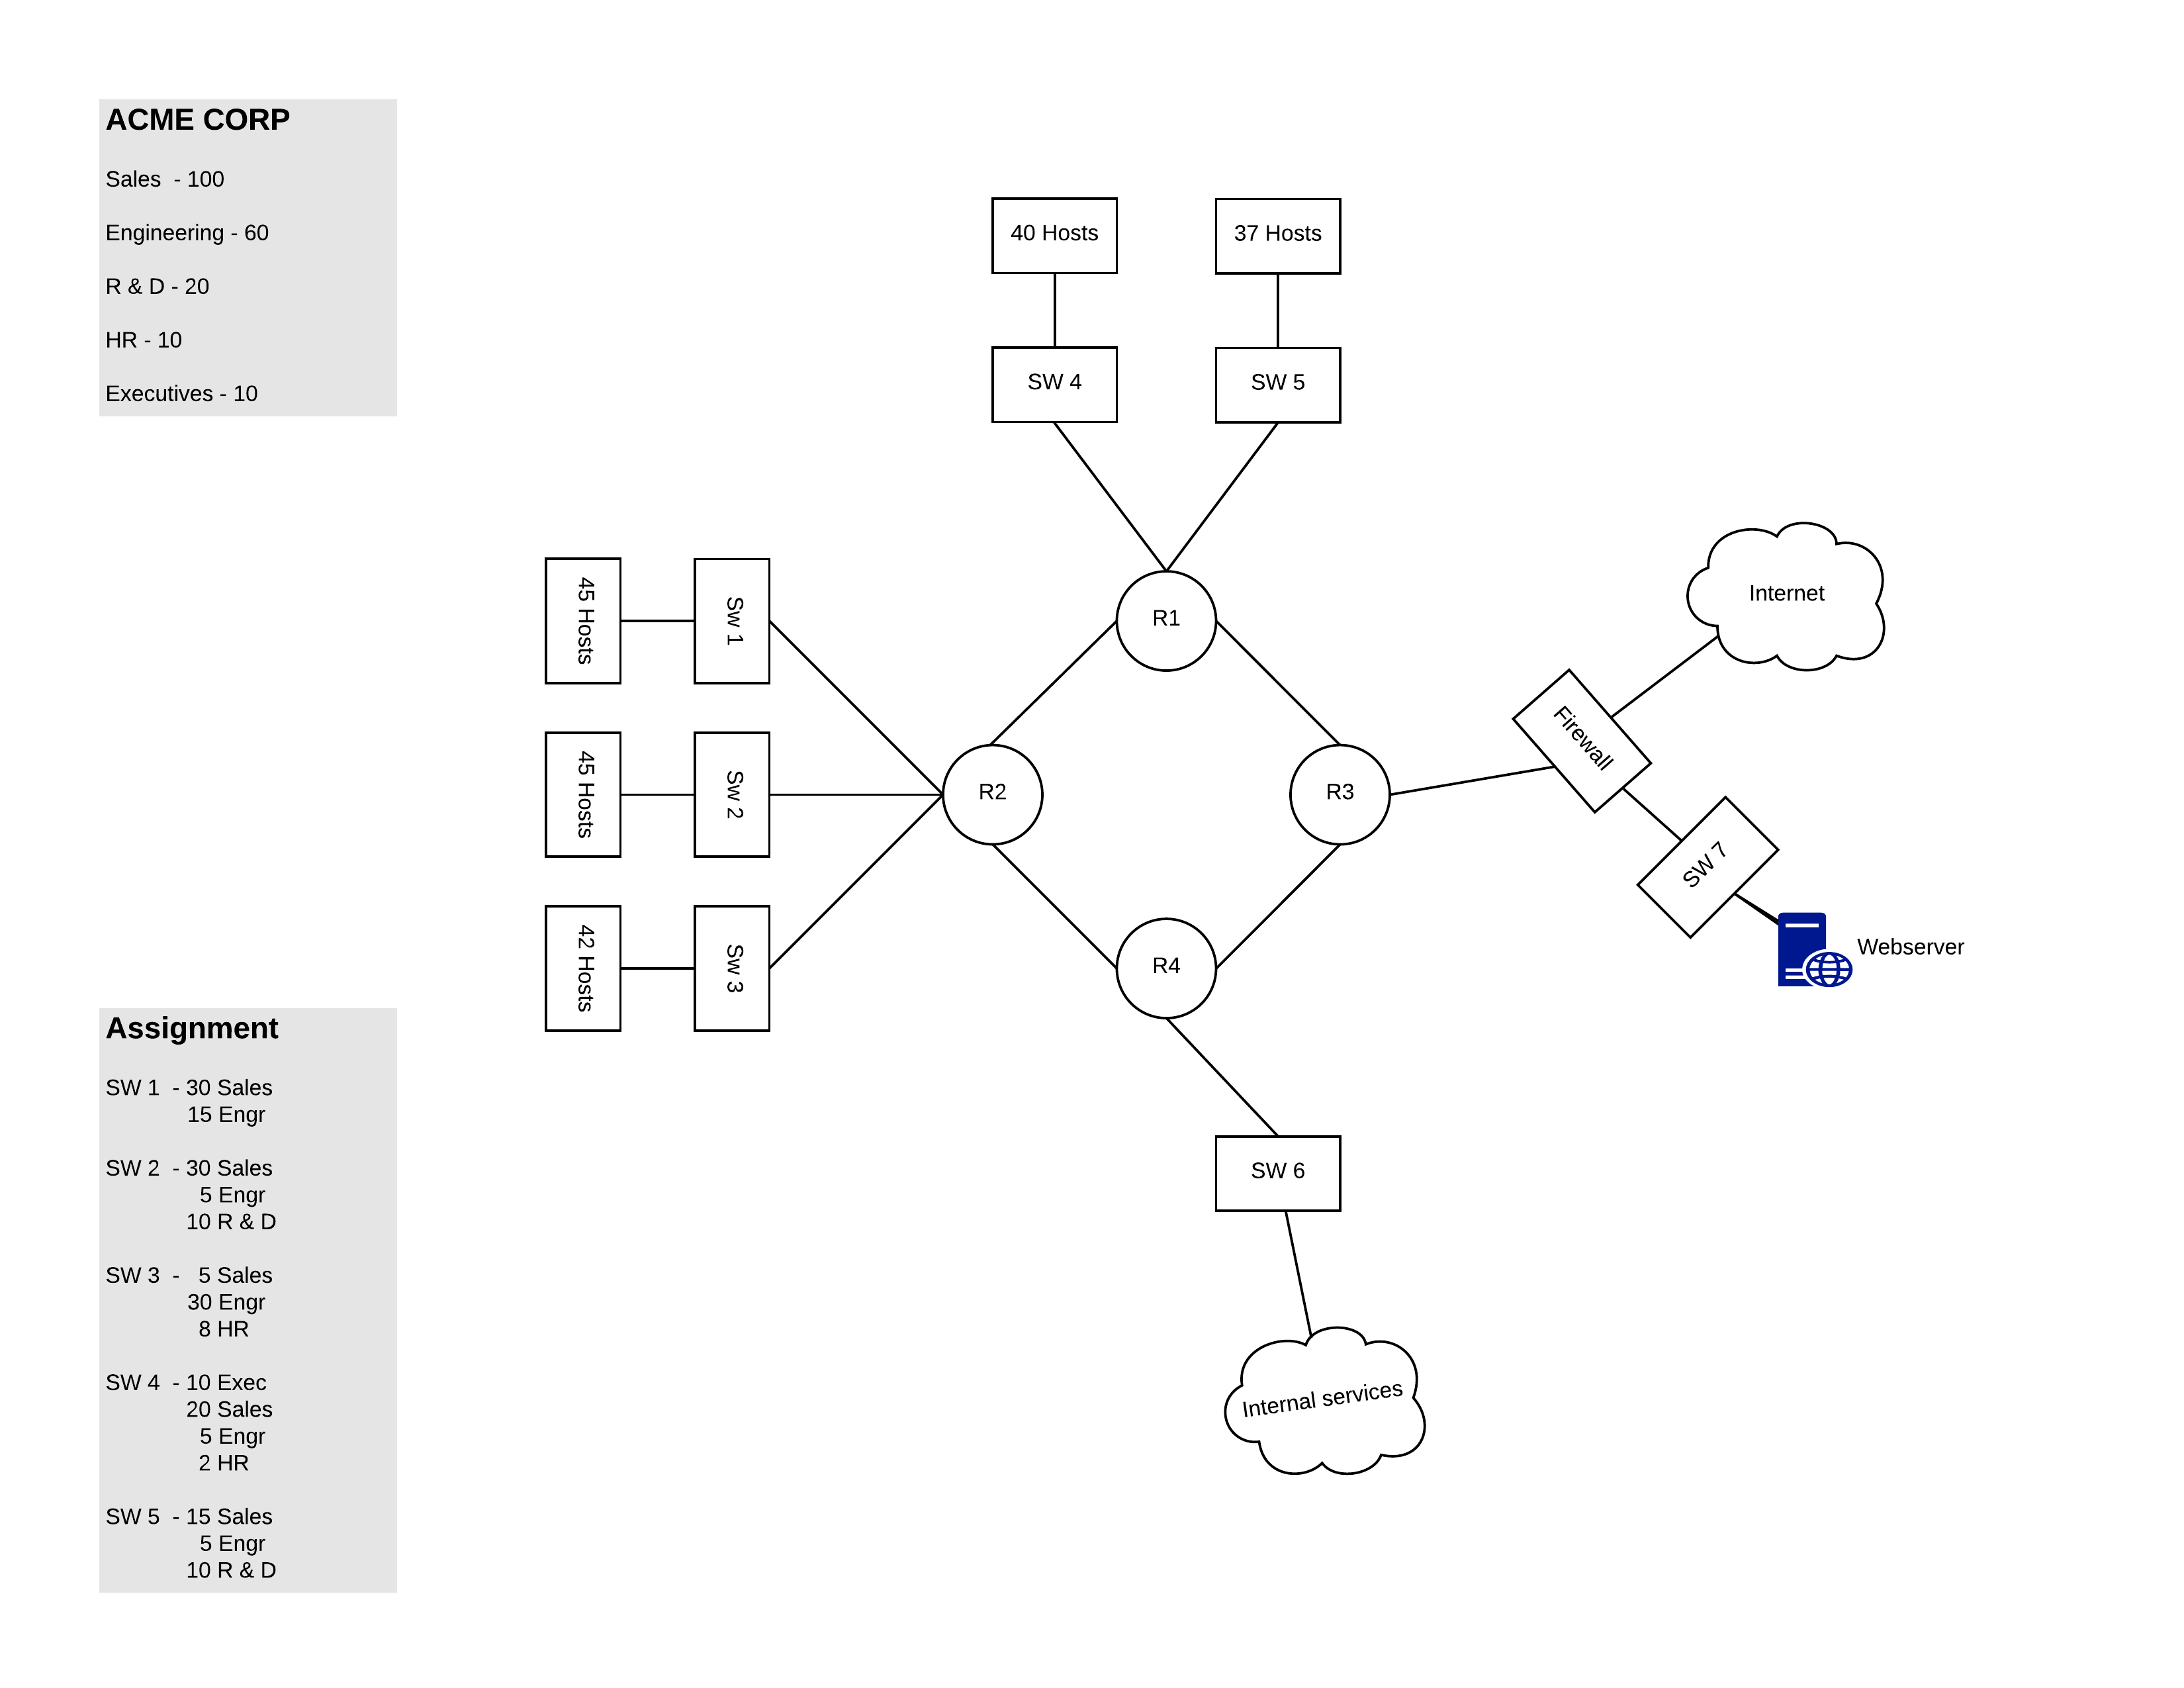
\includegraphics[width=\textwidth]{images/networktopology.png}
	\caption{Subplots from housetrain.data}
\end{figure}
